\documentclass[12pt,a4paper]{article}
\usepackage[utf8]{inputenc}
\usepackage{amsmath}
\usepackage{amsfonts}
\usepackage{amssymb}
\usepackage{graphicx}
\author{Nagy András}
\title{Webes alkalmazások fejlesztése - 1. beadandó}

\begin{document}
\maketitle

\section{Feladat}
Készítsünk egy aukciókkal foglakozó online rendszert, ahol különböző tárgyakra
licitálhatnak a felhasználók.
A  webes  felületet  a  licitálók  használhatják  a 
tárgyak  megtekintésére,  illetve 
ajánlattételre.
\begin{itemize}
\item A  főoldalon  a  legutoljára  meghirdetett  20 tárgy listázódik (név,  hirdető,jelenlegi licitösszeg), de lehetőségünk van kategóriánként megtekinteni az összes(még  aktív)  hirdetést. Egy  oldalon  legfeljebb  20  tárgy  látható  (a 
meghirdetés dátuma szerint csökkenő sorrendben), 
az oldalak között lapozni lehet. A lista szűrhető név(
részlet)-re. A tárgyat kiválasztva megjelennek a 
részletes adatok (kép, leírás, lezárás és meghirdetés 
dátuma , aktuális licit).
\item A licitálónak előbb regisztrálnia kell az oldalon (név, telefonszám,e-mail cím,felhasználónév, jelszó, megerősített jelszó), majd ezt követően bejelentkezhet. A bejelentkezett felhasználó kijelentkezhet.
\item Bejelentkezést  követően érhető  el  a  licitálás  minden  aktív  tárgynál. Licitáláshoz ki 
kell jelölni a tárgyat és meg kell adni az összeget. Első licit esetén az  összegnek a  minimális  licitnek  kell  lennie, később  pedig mindenképpen nagyobbnak kell lennie a korábbi liciteknél. Egy felhasználó tetszőlegesen sokszor licitálhat egy tárgyra. A licitet visszavonni nem lehet.
\item A felhasználó külön listázhatja azokat a tárgyakat, amelyekre legalább egyszer 
licitált. A listában külön megjelöljük az aktív tárgyakat, valamint azokat, ahol 
vezeti a licitet
\end{itemize}

A  grafikus  felületet  az  akciók  hirdetői  használhatják  új  tárgyak  felvitelére, 
valamint a licitálás helyzetének lekérdezésére.

\begin{itemize}
\item Hirdetőként bejelentkezhetünk az alkalmazásba a felhasználónév és a jelszó megadásával, majd ezt követően lehetőségünk van a meghirdetett tárgyak követésére, új tárgy felvitelére, valamint kijelentkezésre.
\item Új tárgy felvitelekor megadjuk az elnevezést, a kategóriát, a leírást, a kezdő licitösszeget, a licitálás lezárásának dátumát, továbbá feltölthetünk egy képet is a tárgyhoz.
\item A  meghirdetett  tárgyak  (a  licitálás  lezárási  ideje  szerint)  listázódnak,  és minden tárgynál megjelenik, hogy jelenleg mennyit ajánlottak 
érte. A tárgyat kiválasztva  megkapjuk  az  összes  információt  képpel  együtt,  valamint  az összes addigi licitet (dátum, név, összeg). Lehetőségünk van a licit azonnali lezárására (csak ha valaki már licitált rá, ekkor az aktuális licitáló viszi a tárgyat)

\end{itemize}

\section{Feladat elemzése}
\subsection{Webes felhasználói felület}
A feladatot a három rétegű, Model-View-Controller architektúrában valósítjuk meg.
\begin{itemize}
\item Az adatok tárolásához, és a felhasználó kezeléshez létrehozunk egy adatbázist, melyben a tárgyak, a licitek, valamit a felhasználók adatait tárolhatjuk. Az adatbázis modelljét az AuctionPortalEntities entitás modell biztosítja.
\item Az oldal egységes megjelenítésért létrehozunk egy megosztott megjelenítőt, melyben be és kijelentkezhetünk, láthatjuk a tárgyakat kötegórák szerint és szűrhetünk is rájuk.
\item A Home könyvtár alatt létrehozzuk a tárgyak listázásért felelős nézetet, valamint az adott tárgy részletei nézetet.
\item Külön nézetet hozunk létre a licitáláshoz, a regisztrációhoz és a bejelentkezéshez. Mindezekhez létrehozunk egy-egy nézetmodellt, melyben eltárolhatjuk a felhasználó által kitöltött információkat.
\item A kontrollerek felelőssége csökkentése érdekében létrehozunk két funkcionalitásért felelős osztályt, az AccounstServicet-t, mely a felhasználói műveltekért felelős, valamint az AuctionService-t, amely a konzisztens licitálást biztosítja, valamint a megfelelő licitek és tárgyak elérést biztosítja.
\item Azon funkciókat, melynek minden kontrollernek  végre kell hajtania, mint a ketegóriák meghatározása, kiemeljük egy bázis kontrollerbe.
\item Külön kontroller felel a felhasználói műveletekért, valamint a licitálás kezeléséért.
\end{itemize}

\subsection{Grafikus kliensfelület}
\begin{itemize}
\item Az adminisztratív grafikus felületet, mely a WebApi-val kommunikál, MVVM architektúrában valósítjuk meg.
\item Elhelyezünk rajta két főmenüt, egyet a hirdetések karbantartásához, valamint egy adminisztrációs menüt, melyben a hirdetőknek lehetőségük van bejelentkezni, kijelenetezni, valamint lehetőségünk van új hirdetőt hozzáadni.
\item Lehetőségünk van új hirdetést hozzáadni, melyre létrehozunk egy külön nézetet(ItemEditorVidnow), valamint lezárni egy kijelölt hirdetést, amennyiben legalább egy licitáló van rá.
\item A hozzáadott hirdetésekhez felvehetünk új képeket, valamint törölhetjük a meglévőket.
\item Egy hirdetés kijelölése hatására megjelenítjük a hozzátartozó képeket, valamint listázzuk a rajtuk lévő liciteket.
\item A hirdetések módosítása aszinkron módon történik.
\end{itemize}

\subsection{Webszolgáltatás}
\begin{itemize}
\item A webszolgáltatást ASP.NET WebApi segítségével valósítjuk meg.
\item Felveszünk egy kontrollert az adminisztrációs műveletek(AccountController), a hirdetések(ItemsController), kategóriák(CategoryController), valamint a képek kezelésére(ItemImagesController).
\end{itemize}

\section{Felhasználói estek}
\subsection{Webes felület}
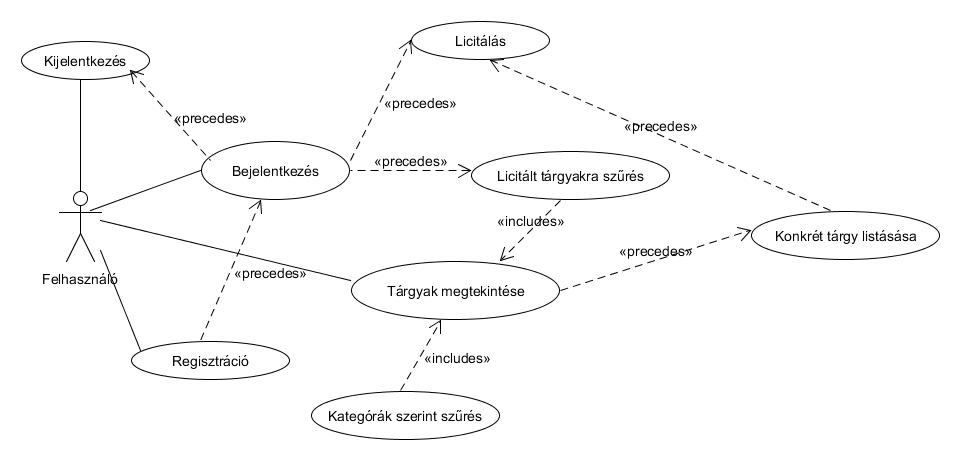
\includegraphics[scale=0.5]{felhasznaloi_diag.jpg}

\subsection{Adminisztratív kliens}
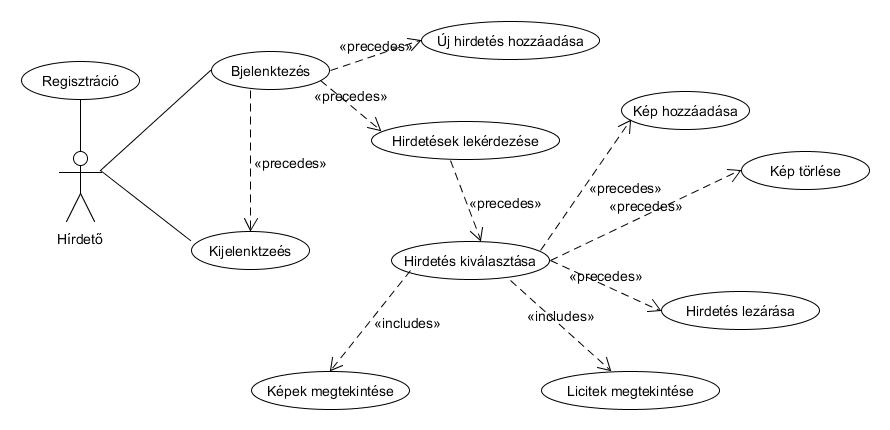
\includegraphics[scale=0.5]{felhasznalo_diag2.jpg}


\section{A rendszer szerkezete}
\subsection{Komponensek}
Az MVC acthitektúrának megfelelően a programnak 2 fontos komponense van.
\begin{itemize}
\item Az adatbázis felelős a rendszer által használt adatok, és a felhasználó információk tárolására. Az adatbázishoz való kapcsolódást az ADO.NET Entity Freamwork segítségével biztosítjuk.
\item A webes alkalmazási felület ASP.NET-ben MVC architektúrával megvalósítva, amely tartalmaz felhasználói nézeteket és ehhez kapcsolódó nézetmodelleket, kontrollereket, valamint az adatbázis modelljét, és a funkcionalitásért felelős kiszolgáló osztályokat.

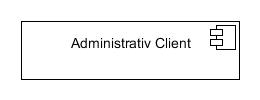
\includegraphics[scale=0.5]{komponens_diagram.jpg}

\end{itemize}
\subsection{Osztályok}
\subsection{Webes felhasználói feület}
\begin{itemize}
\item A Models névtéren belül helyezkednek el a nézetmodelleket, az adatbázis modell, valamint az aukciót és a felhasználói műveletek végző osztályok.
\item A Contorllers névtéren belül a kontrollerek helyezkednek el. A program 3 különböző kontrollere oszlik, valamint a közös funkcionalitást biztosító bázis kontrollere.
\item A View-en belül helyezkedik el a közös megjelenítésért felelős nézet, a tárgyak listázásáért felelős főoldali nézet,  a be-ki jelenkezesértét és a regisztrációért felelős nézetek, valamint a tárgyak részleteit megadó, és a licitálás felület
\end{itemize}
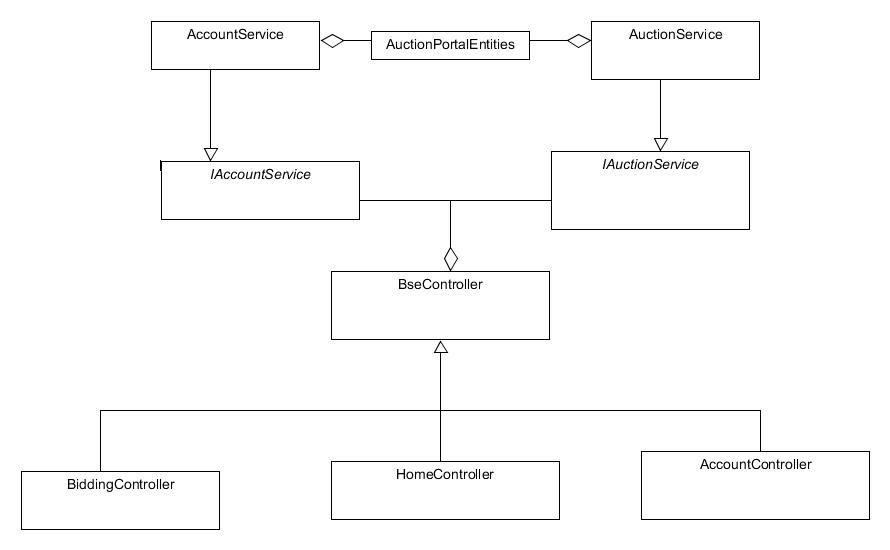
\includegraphics[scale=0.5]{osztaly_szerkezet.jpg}

\subsection{Adminisztratív kliens}

\subsection{Webszolgáltatás}

\section{Adatbázis felépítése}
\begin{itemize}
\item Az adatbázisban tároljuk az egyes meghirdetett tárgyakat, és a hirdetéshez kapcsolódó információkat.
\item A felhasználó adatokat
\item AZ összes ajánlatot, melyben benne van az ajánlat összege, dátuma, tárgya, és az ajánlatot megtett felhasználó.
\item A tárgyakhoz tartozó képeket.
\item Az egyes tárgyak kategóriáját.
\end{itemize}
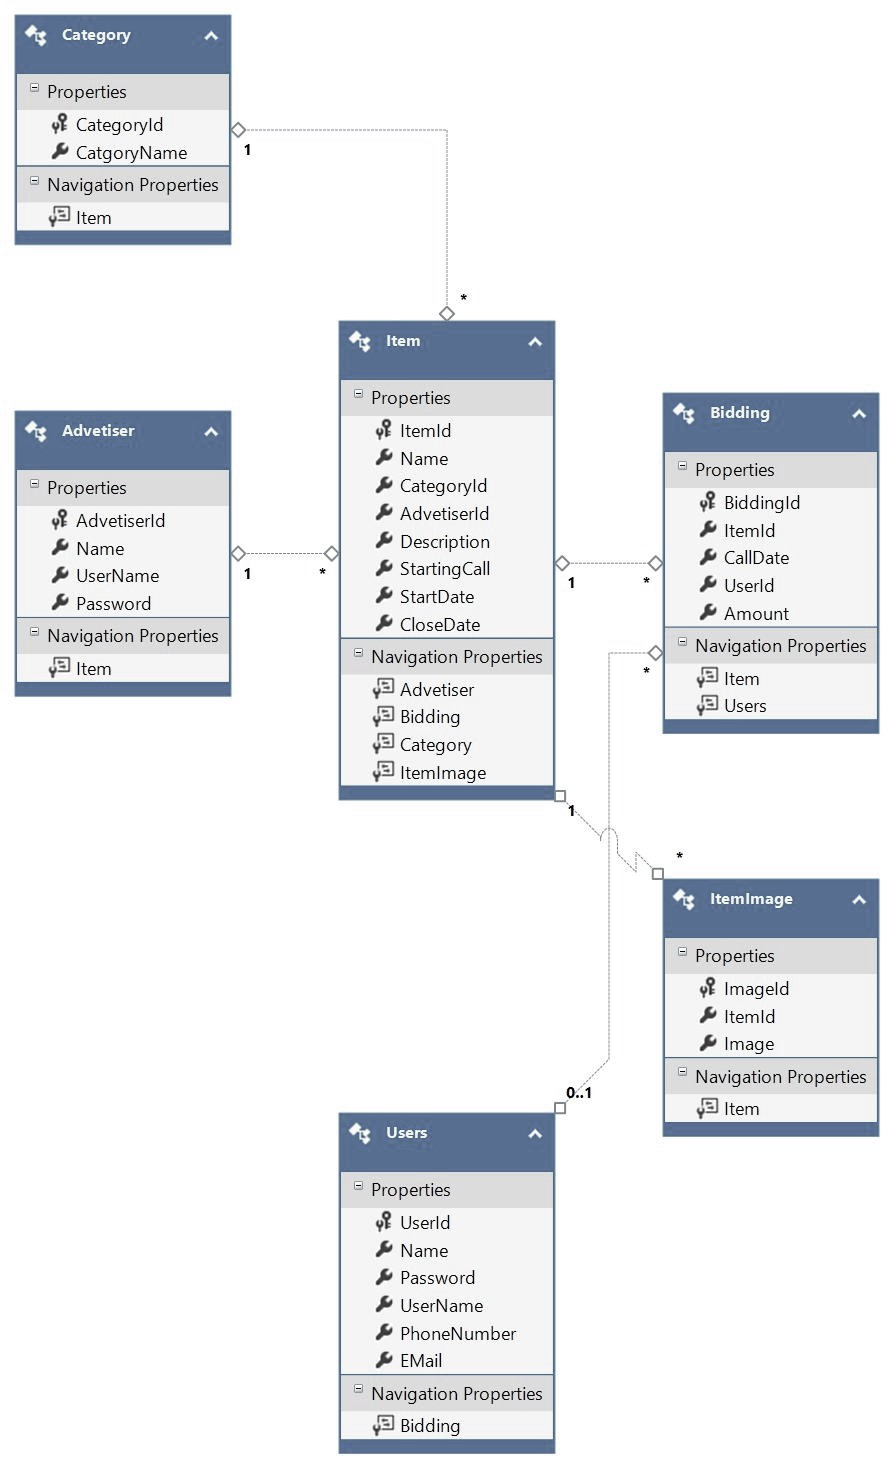
\includegraphics[scale=0.5]{entity_connect.jpg}

\section{Tesztelés}
A webszolgáltatás funkcionalitását egységtesztek segítségével ellenőriztük.

\end{document}